\section{Inductor Design}

In this part, I have designed an inductor with a toroidal core, whose datasheet is given in Figure \ref{datasheet}. \\

\begin{figure}[H]
\hspace{1.5cm}
\centering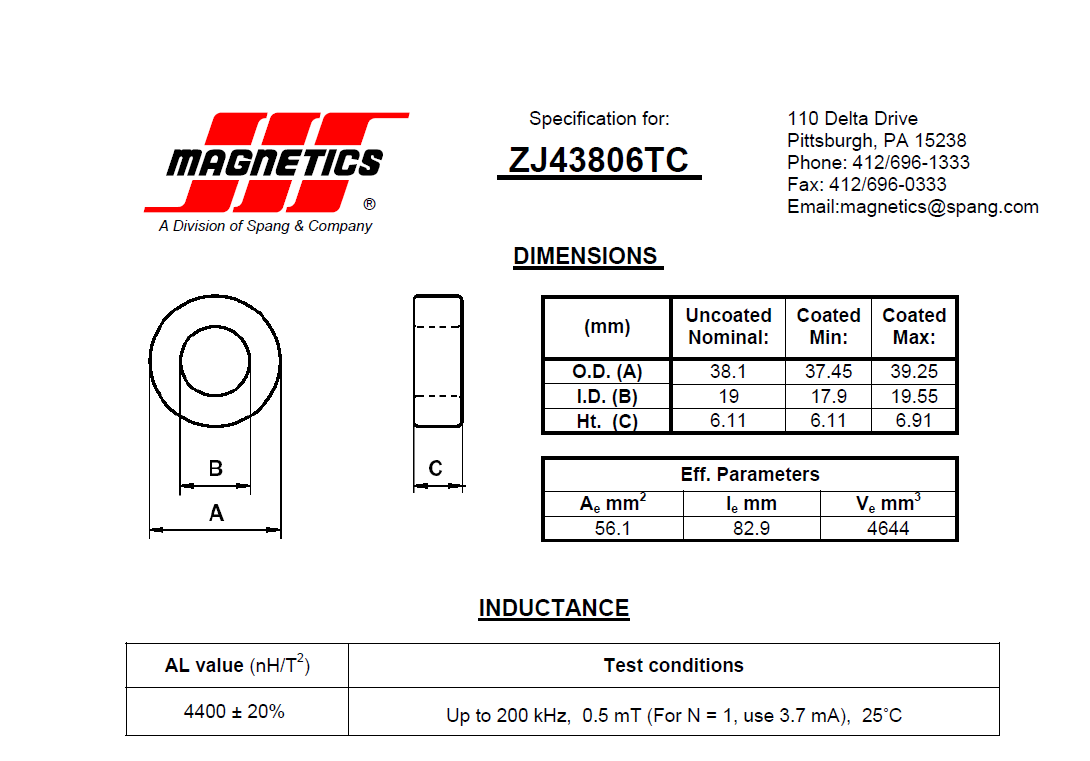
\includegraphics[width=4.5in]{datasheet.PNG}\\
\caption{Datasheet of the Toroidal Core}
\label{datasheet}
\end{figure} 


I chose the number of turns as 15, and Dc current as 0.3 A, in order to obtain N.I= 4.5 A.turns, which makes the inductor operate in linear region, but close to saturation. These choices are verified by calculating, calculations are as follows:\\

$$\dfrac{B*L_{eff}}{\mu_{0}*\mu_r}=N*I$$
$$B=\dfrac{4.5*5000*4*\pi*10^{-7}}{0.0829}=0.341 T$$
\\

Analytical calculations of inductance (with MATLAB code) are given below. It should be considered that BH curve data used in non-linear material calculations does not belong to the material that I have chosen. Its relative permeability is around 4000, where that of my toroid of choice is 5000. An additional difference is also expected in analytical calculations because of this fact.\\ 

\sloppy
\definecolor{lightgray}{gray}{0.5}
\setlength{\parindent}{0pt}

  
    
\subsection*{Part A}

\subsubsection*{Parameters}

\begin{verbatim}
in_dia= 19; %mm
in_rad=in_dia/2*1e-3;
out_dia= 38.1; %mm
out_rad=out_dia/2*1e-3;
ht= 6.11; %mm

Leff=82.9; %mm
Aeff=56.1; %mm^2

N=15 ;% turns
I=0.3; % A

mu_r=5000;
mu_0=4*pi*1e-7;

AL=4400; %nH/turns^2
\end{verbatim}


\subsubsection*{Analytical Calculations}

\begin{verbatim}
%
% # 1

reluctance=Leff*1e-3/(Aeff*1e-6*mu_r*mu_0);

L=N^2/reluctance; %H

fprintf('Inductance assuming homogeneous distribution is %d H. \n', L);

% # 2
% In this part, H.dl should be integrated over over the cross-section of
% coaxial circles with radii from in_dia/2 to out_dia/2.
% H*2*pi*(out_rad-in_rad)=N.I

index=linspace(in_rad,out_rad,500);
for i=1:numel(index)

    H(:,i)=N*I/(2*pi*index(:,i));
    B(:,i)=mu_0*mu_r*H(:,i); %T
    Phi(:,i)=B(:,i)*ht*1e-3*(out_rad-in_rad)/500; %Wb
end

tot_phi=0;

for k=1:500

   tot_phi=tot_phi+Phi(:,i);

end

L_2=tot_phi*N/I;

fprintf('Inductance assuming non-homogeneous distribution is %d H. \n', L_2);
%
% # 3_1
%
I_2=I*1.5;

H_2=N*I_2/(Leff*1e-3);

B_2=interp1(B_nl,H_nl,H_2);

phi_2=Aeff*1e-6*B_2;

L_3=N*phi_2/I_2;

fprintf('Inductance assuming homogeneous distribution & non-homogeneous material is %d H. \n', L_3);

%
% # 3_2
%


index=linspace(in_rad,out_rad,500);
for i=1:numel(index)

    H_3(:,i)=N*I_2/(2*pi*index(:,i));
    B_3(:,i)=interp1(B_nl,H_nl,H_3(:,i));
    Phi(:,i)=B_3(:,i)*ht*1e-3*(out_rad-in_rad)/500; %Wb
end

tot_phi=0;

for k=1:500

   tot_phi=tot_phi+Phi(:,i);

end

L_4=tot_phi*N/I_2;

fprintf('Inductance assuming non-homogeneous distribution & non-homogeneous material is %d H. \n', L_4);

%
% # 4
%

rel_gap=2e-3/(mu_0*Aeff*1e-6);
rel_core=(Leff-2)*1e-3/(Aeff*1e-6*mu_r*mu_0);
rel_tot=rel_gap+rel_core;

L_5=N^2/rel_tot;

fprintf('Inductance of the gapped core assuming homogeneous distribution is %d H. \n', L_5);

%
% # 5
%

% In this part, we may assume the fringing flux is considerable for an area
% of 2 mm (the length of airgap) to the left and to the right of the
% airgap. Therefore we may assume the equivalent reluctance of the magnetic
% circuit as R_core in series with (R_gap_left||R_gap||R_gap_right). This
% approach is not a reliable one, nevertheless it may give us an idea.

rel_gap_side=2e-3/(mu_0*2e-3*ht*1e-3);
rel_tot_2=rel_core+(1/rel_gap_side+1/rel_gap+1/rel_gap_side)^(-1);

L_6=N^2/rel_tot_2;

fprintf('Inductance of the gapped core including fringing flux is %d H. \n', L_6);
\end{verbatim}

        \color{lightgray} \begin{verbatim}Inductance assuming homogeneous distribution is 9.566889e-04 H. 
Inductance assuming non-homogeneous distribution is 6.891791e-04 H. 
Inductance assuming homogeneous distribution & non-homogeneous material is 5.383088e-04 H. 
Inductance assuming non-homogeneous distribution & non-homogeneous material is 5.027784e-04 H. 
Inductance of the gapped core assuming homogeneous distribution is 7.867304e-06 H. 
Inductance of the gapped core including fringing flux is 1.125535e-05 H. 
\end{verbatim} \color{black}
    

\subsection*{Part B}

\begin{enumerate}
\item
Mesh plots, B field distribution, distribution of B vectors and flux line distribution of the toroid, assuming linear magnetic material properties, are given below on Figures \ref{mesh1}-\ref{flux1}. Note that thin copper layer inside the toroid is excited with positive 4.5 A.t and the one that is at the outside of the toroid is excited with negative 4.5 A.t.\\

\begin{figure}[H]
\hspace{1.5cm}
\centering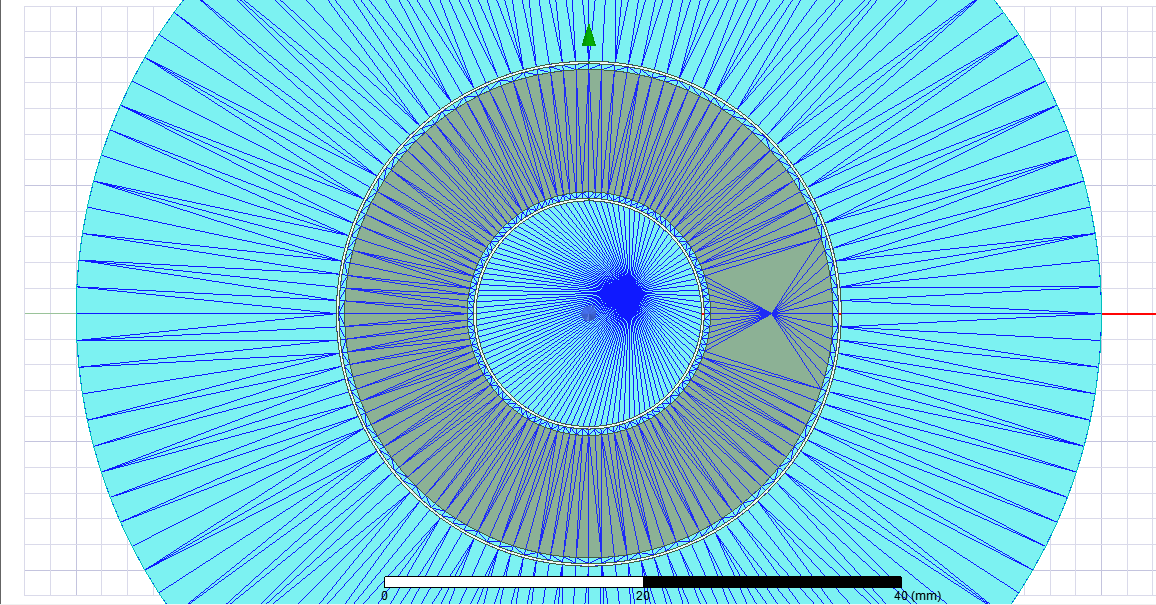
\includegraphics[width=4.5in]{mesh.PNG}\\
\caption{Mesh Operations on the Toroid}
\label{mesh1}
\end{figure} 

\begin{figure}[H]
\hspace{1.5cm}
\centering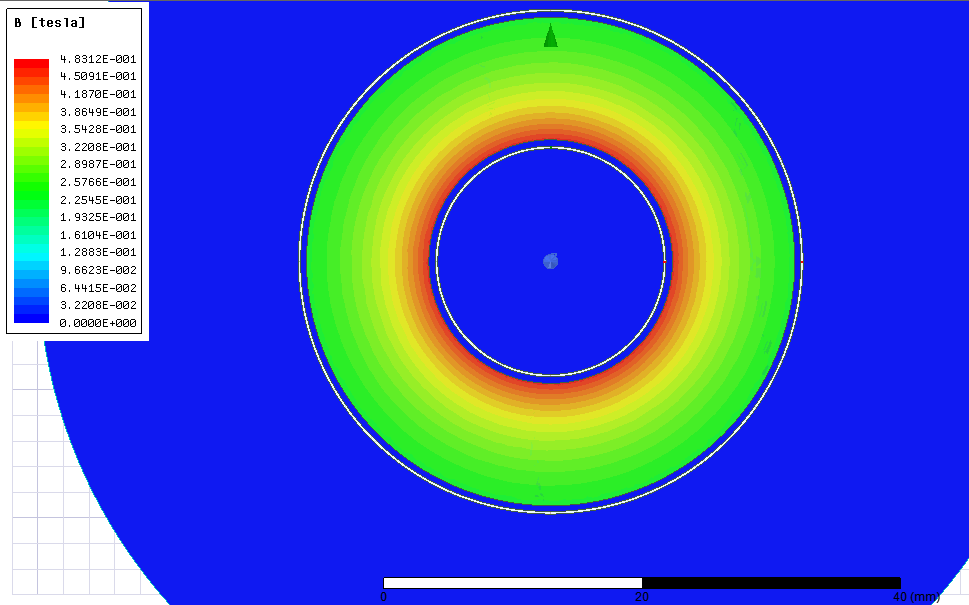
\includegraphics[width=4.5in]{b_field.PNG}\\
\caption{B Field Distribution in the Inductor}
\label{b1}
\end{figure} 

\begin{figure}[H]
\hspace{1.5cm}
\centering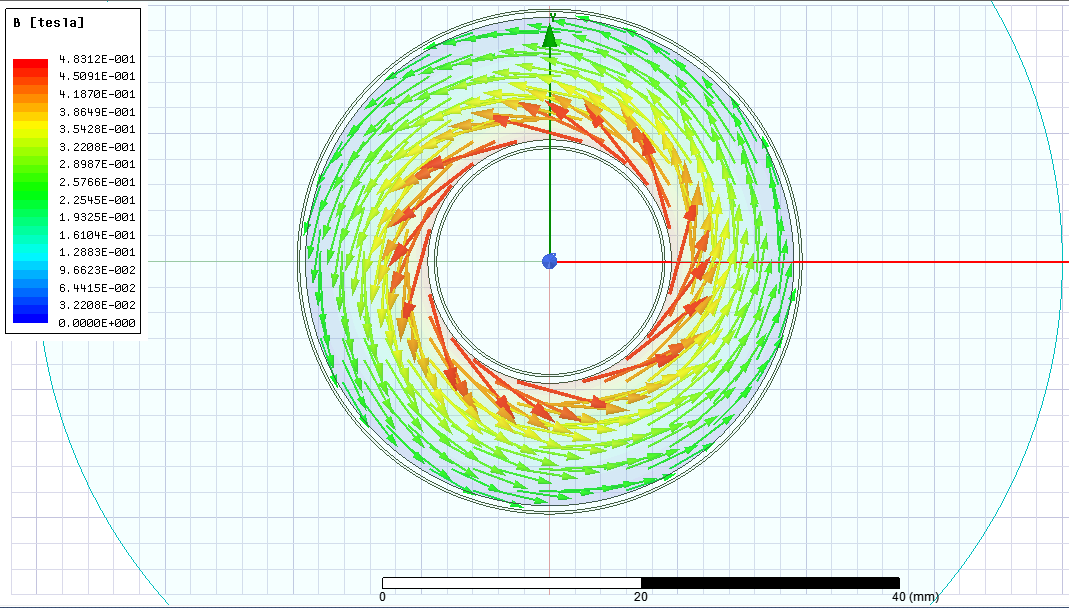
\includegraphics[width=4.5in]{b_vector.PNG}\\
\caption{B Vectors in the Inductor}
\label{bvec1}
\end{figure}

\begin{figure}[H]
\hspace{1.5cm}
\centering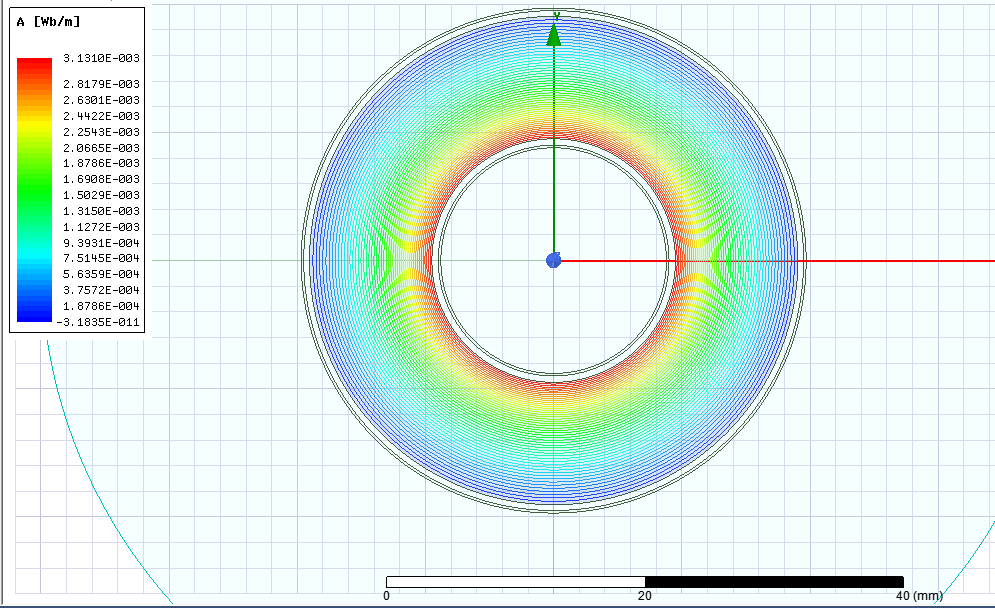
\includegraphics[width=4.5in]{flux_line.PNG}\\
\caption{Flux Lines in the Toroidal Core}
\label{flux1}
\end{figure} 

\item
Inductance is calculated on the line from inner radius to outer radius, using the formula given below:\\

$$L=\dfrac{N*B*A}{I}$$\\

where A is denoted by the line, since the simulation is 2D.\\

To calculate the leakage inductance, same approach is used, (with a longer line crossing both inner and outer sides of the inductor) however no leakage is observed in this case. Inductance values are given on Figures \ref{ind1} and \ref{leak1}, below.

\begin{figure}[H]
\hspace{1.5cm}
\centering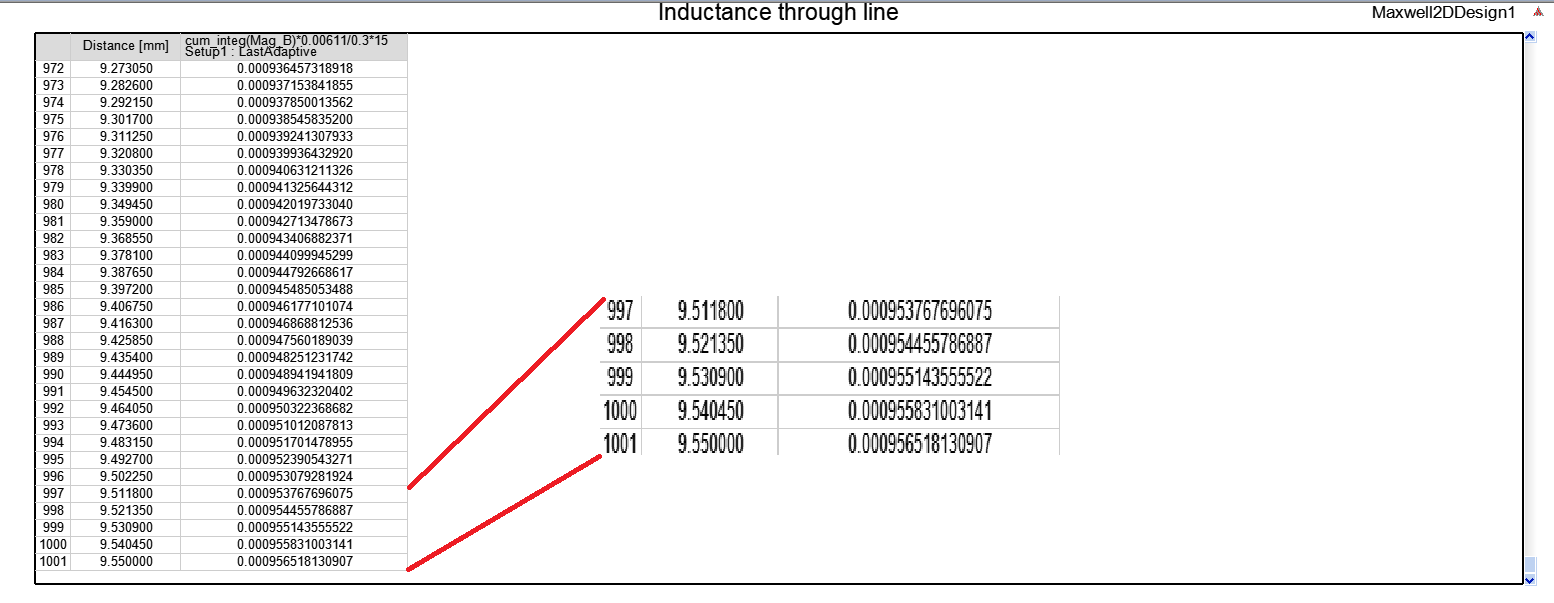
\includegraphics[width=4.5in]{linear_inductance.PNG}\\
\caption{Inductance with Linear Material Properties}
\label{ind1}
\end{figure} 


\item
Here, the major observation is the saturation of the core. Also, there is a considerable drop in inductance. \\

\begin{figure}[H]
\hspace{1.5cm}
\centering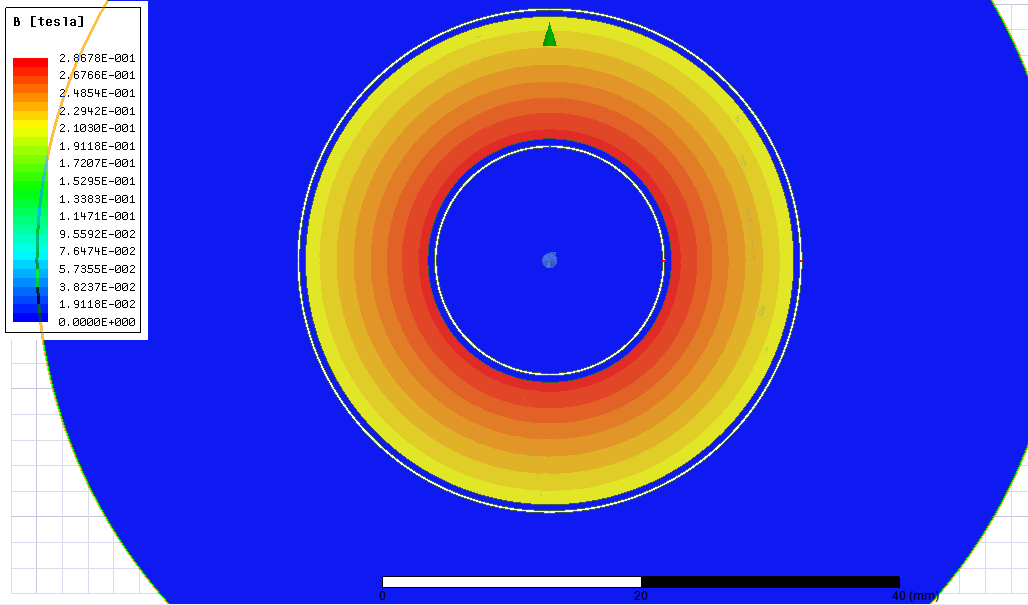
\includegraphics[width=4.5in]{b_field_nonlinear.PNG}\\
\caption{B Field Distribution in the Inductor with Non-Linear Material Properties}
\label{b2}
\end{figure} 

\begin{figure}[H]
\hspace{1.5cm}
\centering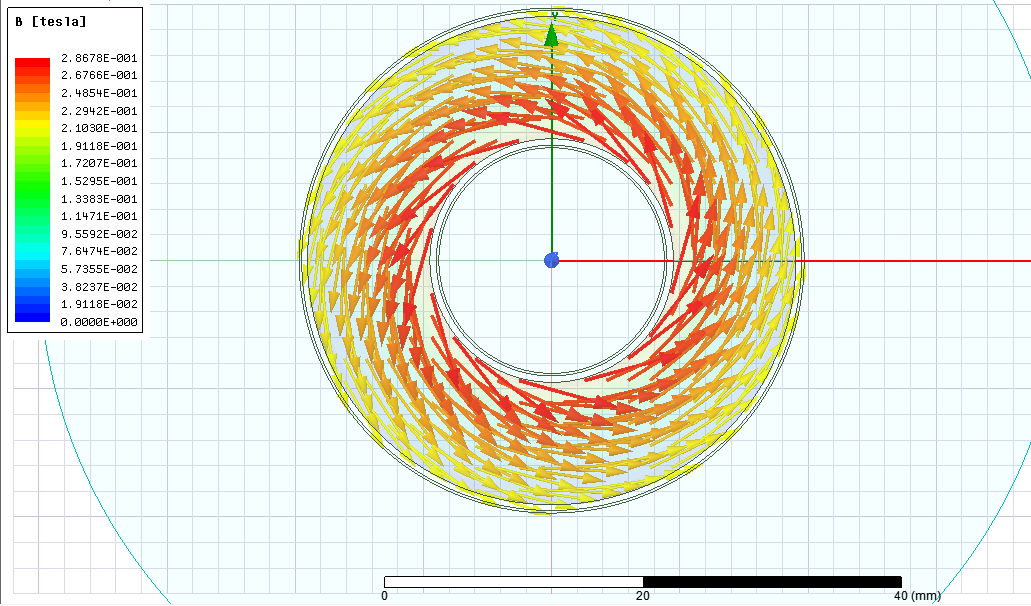
\includegraphics[width=4.5in]{b_vector_nonlinear.PNG}\\
\caption{B Vectors in the Inductor with Non-Linear Material Properties}
\label{bvec2}
\end{figure}

\begin{figure}[H]
\hspace{1.5cm}
\centering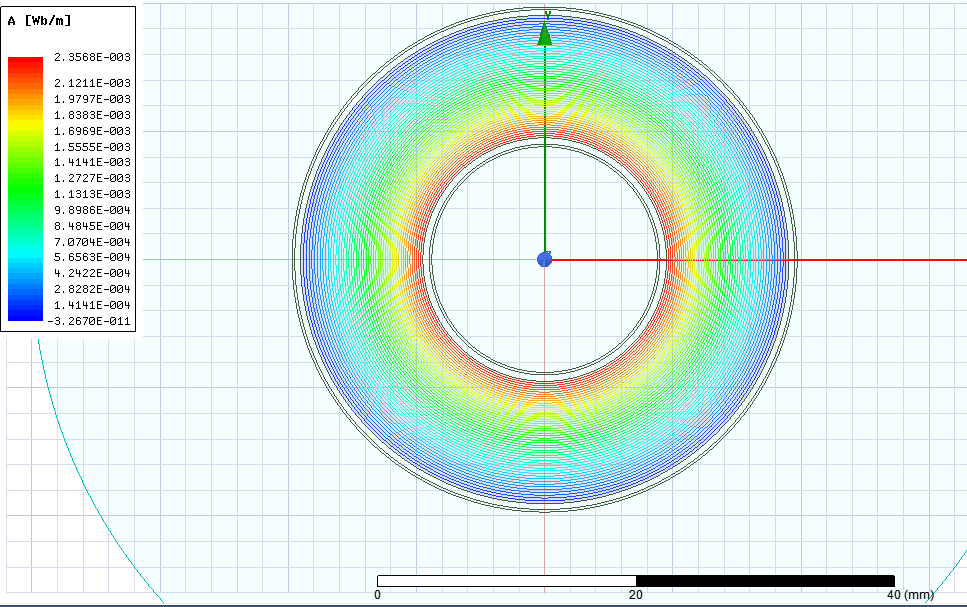
\includegraphics[width=4.5in]{flux_line_nonlinear.PNG}\\
\caption{Flux Lines in the Toroidal Core with Non-Linear Material Properties}
\label{flux2}
\end{figure} 

\begin{figure}[H]
\hspace{1.5cm}
\centering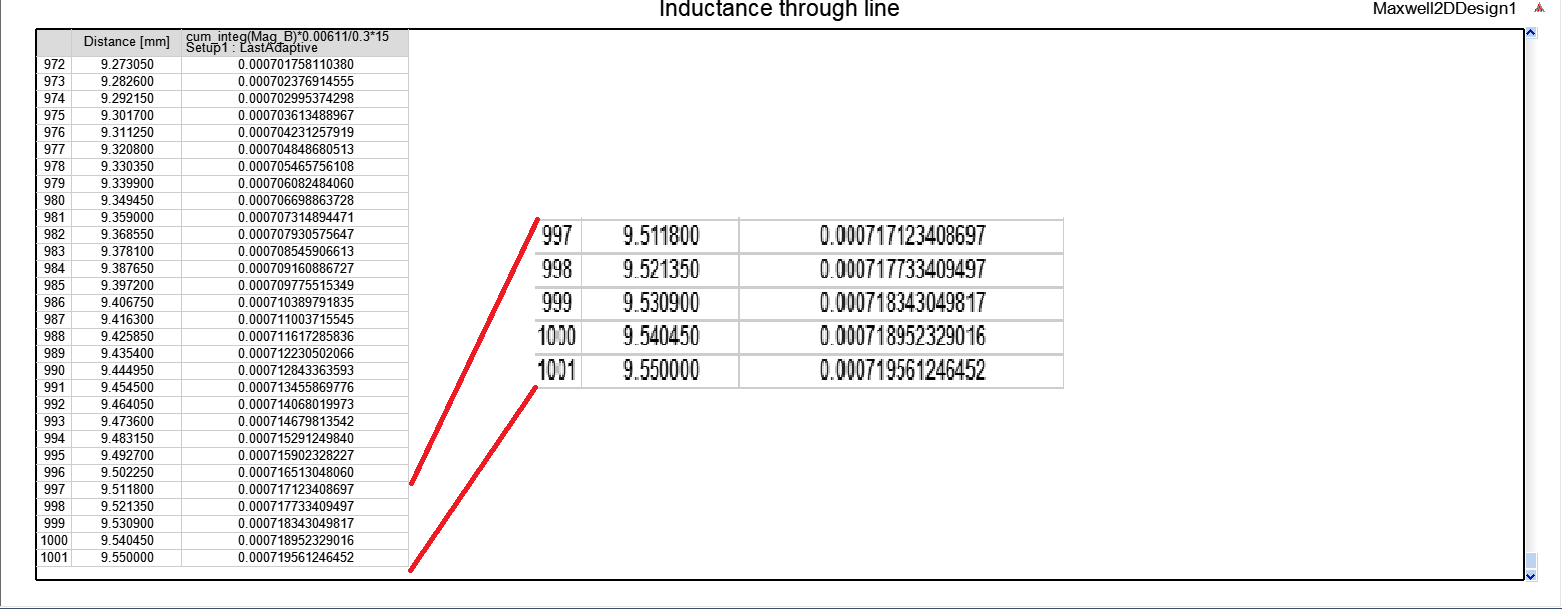
\includegraphics[width=4.5in]{nonlinear_inductance.PNG}\\
\caption{Inductance with Non-Linear Material Properties}
\label{ind2}
\end{figure}

\begin{figure}[H]
\hspace{1.5cm}
\centering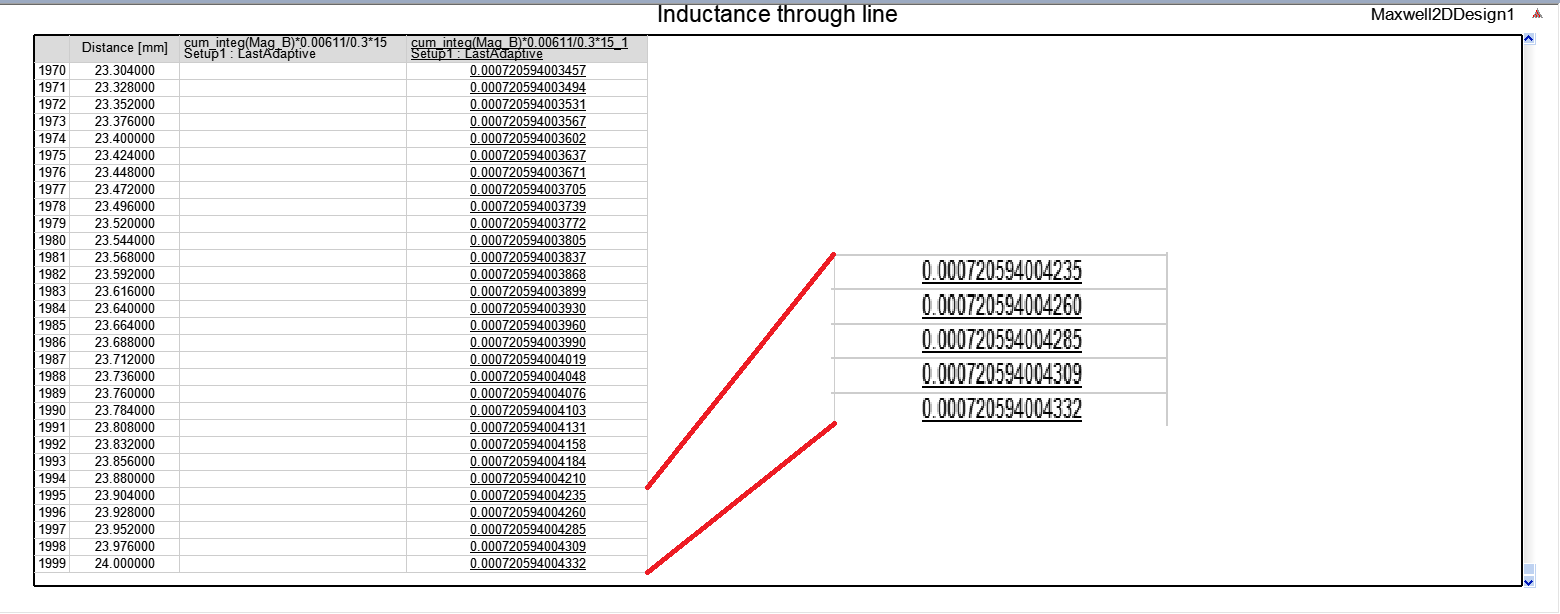
\includegraphics[width=4.5in]{leakage.PNG}\\
\caption{Leakage Included Inductance with Non-Linear Material Properties}
\label{leak1}
\end{figure} 


\item
In this case, airgap introduces a significant increase in reluctance to the system, therefore inductance decreases considerably. Further, we can observe the effect of leakage and fringing flux on Figures \ref{b3}, \ref{bvec3} and \ref{flux3}, which creates leakage inductance. Leakage inductance can be calculated bu subtracting inductance value on Figure \ref{ind3} from overall inductance given in Figure \ref{leak2}. 

\begin{figure}[H]
\hspace{1.5cm}
\centering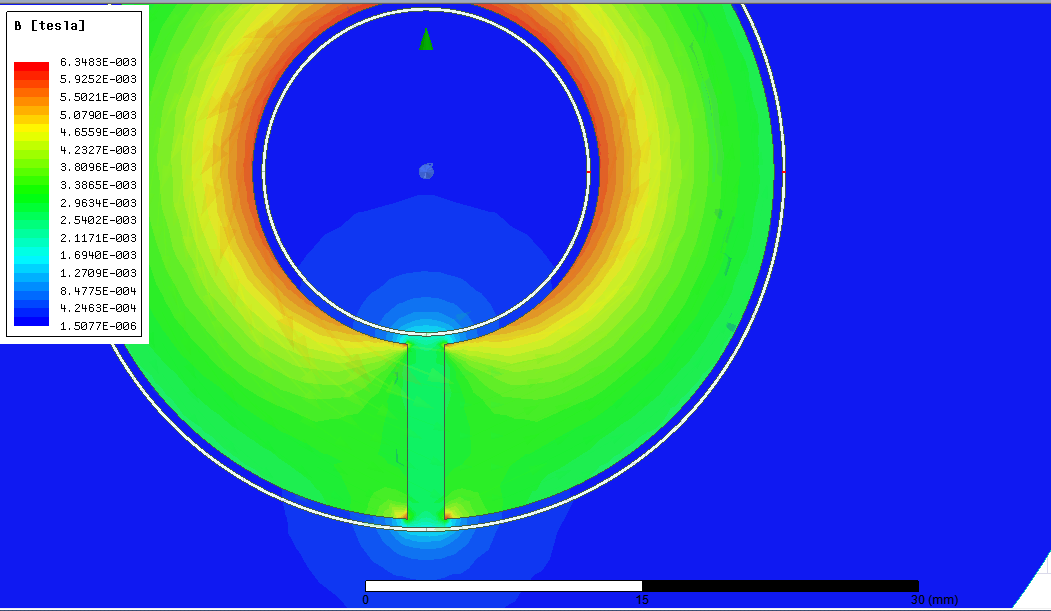
\includegraphics[width=4.5in]{b_field_ag.PNG}\\
\caption{B Field Distribution in the Gapped Inductor with Non-Linear Material Properties}
\label{b3}
\end{figure} 

\begin{figure}[H]
\hspace{1.5cm}
\centering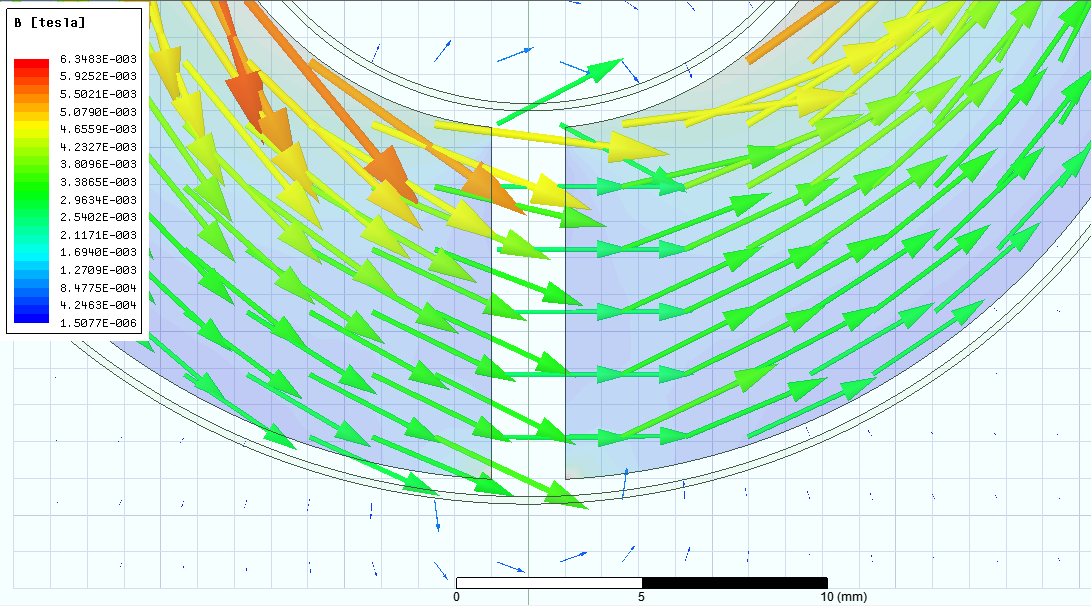
\includegraphics[width=4.5in]{airgap_b_vector.PNG}\\
\caption{B Vectors in the Gapped Inductor with Non-Linear Material Properties}
\label{bvec3}
\end{figure}

\begin{figure}[H]
\hspace{1.5cm}
\centering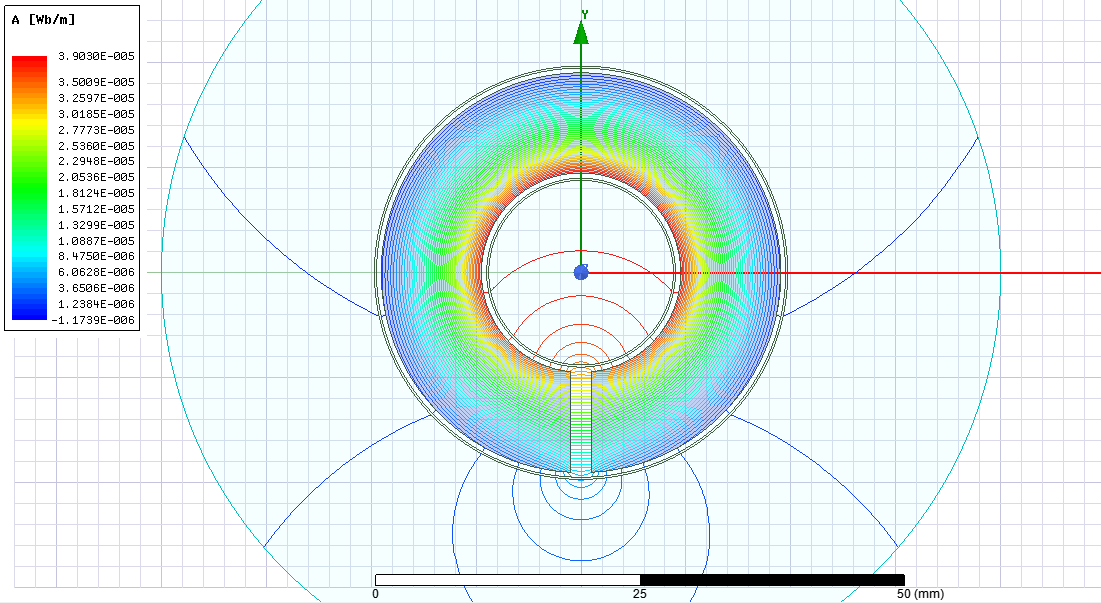
\includegraphics[width=4.5in]{flux_line_ag.PNG}\\
\caption{Flux Lines in the Gapped Toroidal Core with Non-Linear Material Properties}
\label{flux3}
\end{figure} 

\begin{figure}[H]
\hspace{1.5cm}
\centering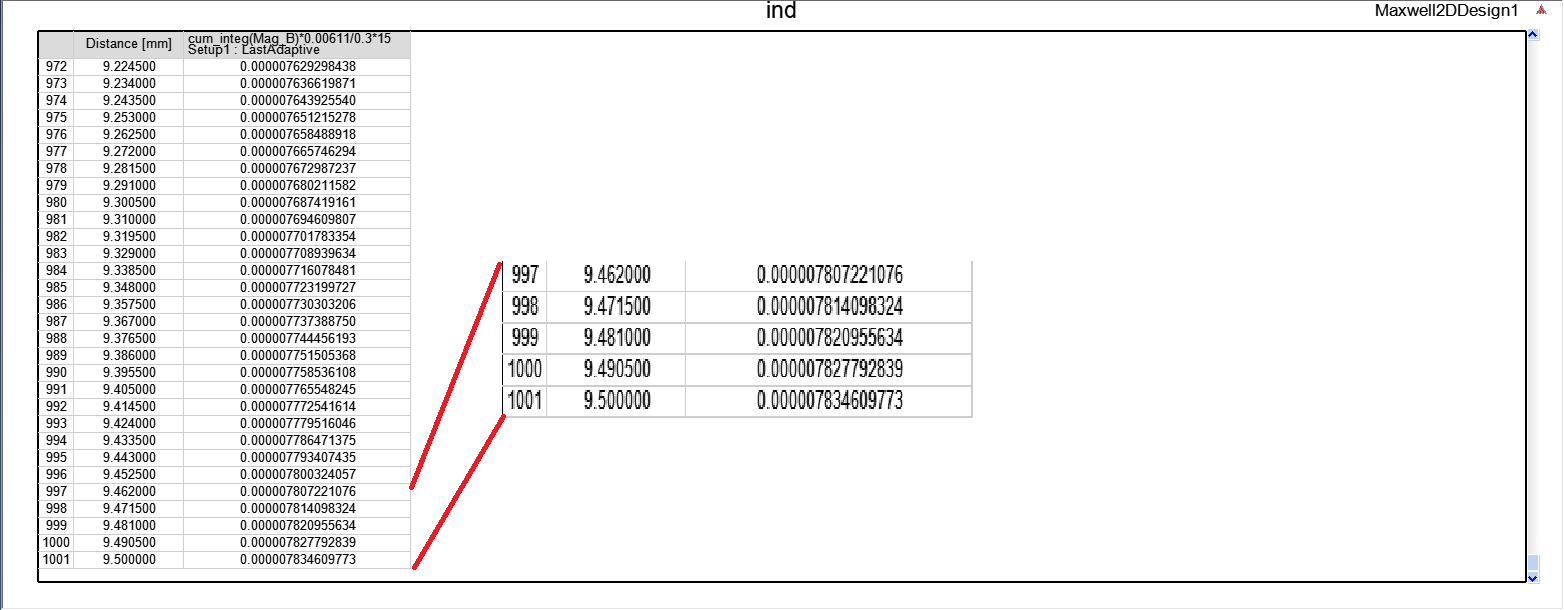
\includegraphics[width=4.5in]{inductance_ag.PNG}\\
\caption{Inductance of the Gapped Core with Non-Linear Material Properties}
\label{ind3}
\end{figure}

\begin{figure}[H]
\hspace{1.5cm}
\centering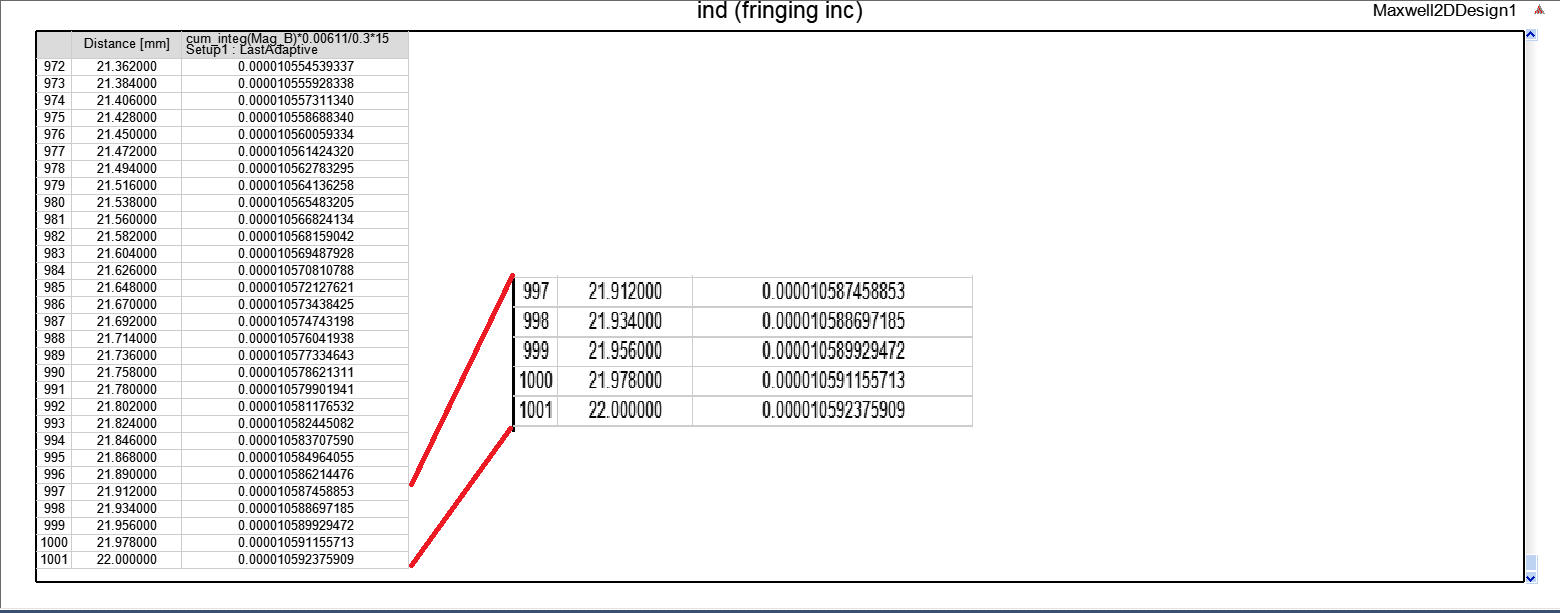
\includegraphics[width=4.5in]{overall_inductance_ag.PNG}\\
\caption{Leakage Included Inductance of the Gapped Core with Non-Linear Material Properties}
\label{leak2}
\end{figure}

\end{enumerate}

\subsection*{Part C}

Below, on Table \ref{compare}, inductance calculation results of both methods are present.

\begin{table}
\centering
\caption{Comparison of Inductance Calculations}
\label{compare}
\begin{tabular}{lllll}
            & FEA         & Analytical  &  &  \\
Linear      & 0.956 mH    & 0.957 mH    &  &  \\
Non-Linear  & 0.720 mH    & 0.538 mH    &  &  \\
With Airgap & 7.83 $\mu$H & 7.87 $\mu$H &  & 
\end{tabular}
\end{table}

Possible discrepancies between these calculations are caused by approximations made in analytical approach. In FEA, as calculations are made for infinitesimal elements and then integrated, it gives us more precise results. However for analytical approach, this is not possible. Hence, for calculations such as non-linear or non-homogeneous material properties, FEA technique is more reliable.\\

If we used 3D FEA instead of 2D, we could also observe the leakage and fringing flux through the cross-section of the core.

